% Copyright 2004 by Till Tantau <tantau@users.sourceforge.net>.
%
% In principle, this file can be redistributed and/or modified under
% the terms of the GNU Public License, version 2.
%
% However, this file is supposed to be a template to be modified
% for your own needs. For this reason, if you use this file as a
% template and not specifically distribute it as part of a another
% package/program, I grant the extra permission to freely copy and
% modify this file as you see fit and even to delete this copyright
% notice. 

\documentclass[aspectratio=169]{beamer}
%\documentclass{beamer}

\setbeamersize{text margin left=10mm, text margin right=10mm}

\defbeamertemplate{headline}{my header}{%
\vskip1pt%
\makebox[0pt][l]{\,\insertshortauthor}%
\hspace*{\fill}\insertshorttitle/\insertshortsubtitle\hspace*{\fill}%
\llap{\insertpagenumber/\insertpresentationendpage\,}
}
\setbeamertemplate{headline}[my header]

\usepackage{graphicx}
\usepackage{soul}
\usepackage{tkz-euclide}
\usetikzlibrary{calc}
\usepackage[]{algorithm2e}
\usepackage{changepage}
\usepackage{amssymb}
\usepackage{xcolor}
\usepackage{mathtools}
\usepackage{tcolorbox}
\usepackage{tikz}
\usetikzlibrary{arrows}
\usepackage{tikz-3dplot}
\usepackage{tkz-euclide}
\usepackage{circuitikz}
\usepackage{pgfplots}
\pgfplotsset{width=7cm,compat=1.8}

\usetikzlibrary{positioning}
% \usepackage[math]{cellspace}
% \cellspacetoplimit 4pt
% \cellspacebottomlimit 4pt
%\usetikzlibrary{arrows.meta}
% sqare of half axes
\newcommand{\asa}{3}
\newcommand{\bsa}{1}
\newcommand{\csa}{0.25}
% view angle
\tdplotsetmaincoords{70}{135}

%\setbeamertemplate{itemize items}{-}

%\usepackage{helvet}
\usefonttheme{professionalfonts} % using non standard fonts for beamer
%\usefonttheme{serif} % default family is serif
%\usepackage{fontspec}
%\setmainfont{Liberation Serif}

% There are many different themes available for Beamer. A comprehensive
% list with examples is given here:
% http://deic.uab.es/~iblanes/beamer_gallery/index_by_theme.html
% You can uncomment the themes below if you would like to use a different
% one:
%\usetheme{AnnArbor}
%\usetheme{Antibes}
%\usetheme{Bergen}
%\usetheme{Berkeley}
%\usetheme{Berlin}
%\usetheme{Boadilla}
%\usetheme{boxes}
%\usetheme{CambridgeUS}
%\usetheme{Copenhagen}
%\usetheme{Darmstadt}
%\usetheme{default}
%\usetheme{Frankfurt}
%\usetheme{Goettingen}
%\usetheme{Hannover}
%\usetheme{Ilmenau}
%\usetheme{JuanLesPins}
%\usetheme{Luebeck}
%\usetheme{Madrid}
%\usetheme{Malmoe}
%\usetheme{Marburg}
%\usetheme{Montpellier}
%\usetheme{PaloAlto}
%\usetheme{Pittsburgh}
%\usetheme{Rochester}
%\usetheme{Singapore}
%\usetheme{Szeged}
%\usetheme{Warsaw}

\def\mf{\ensuremath\mathbf}
\def\mb{\ensuremath\mathbb}
\def\lp{\ensuremath\left(}
\def\rp{\ensuremath\right)}
\def\lv{\ensuremath\left\lvert}
\def\rv{\ensuremath\right\rvert}
\def\lV{\ensuremath\left\lVert}
\def\rV{\ensuremath\right\rVert}
\def\lc{\ensuremath\left\{}
\def\rc{\ensuremath\right\}}
\def\ls{\ensuremath\left[}
\def\rs{\ensuremath\right]}
\def\bmx{\ensuremath\begin{bmatrix*}[r]}
\def\emx{\ensuremath\end{bmatrix*}}
\def\bmxc{\ensuremath\begin{bmatrix*}[c]}


\newcommand{\demoex}[2]{\onslide<#1->\begin{color}{black!60} #2 \end{color}}
\newcommand{\demoexc}[3]{\onslide<#1->\begin{color}{#2} #3 \end{color}}
\newcommand{\anim}[3]{\onslide<#1->{\begin{color}{#2!60} #3 \end{color}}}



\title{Linear Systems}

% A subtitle is optional and this may be deleted
\subtitle{Linear Dynamical Systems: Transfer function view}

\author{Sivakumar Balasubramanian}
% - Give the names in the same order as the appear in the paper.
% - Use the \inst{?} command only if the authors have different
%   affiliation.

\institute[Christian Medical College] % (optional, but mostly needed)
{
  \inst{}%
  Department of Bioengineering\\
  Christian Medical College, Bagayam\\
  Vellore 632002
}
% - Use the \inst command only if there are several affiliations.
% - Keep it simple, no one is interested in your street address.

\date{}
% - Either use conference name or its abbreviation.
% - Not really informative to the audience, more for people (including
%   yourself) who are reading the slides online

\subject{Lecture notes on linear systems}
% This is only inserted into the PDF information catalog. Can be left
% out. 

% If you have a file called "university-logo-filename.xxx", where xxx
% is a graphic format that can be processed by latex or pdflatex,
% resp., then you can add a logo as follows:

% \pgfdeclareimage[height=0.5cm]{university-logo}{university-logo-filename}
% \logo{\pgfuseimage{university-logo}}

% Delete this, if you do not want the table of contents to pop up at
% the beginning of each subsection:
\AtBeginSubsection[]
{
  \begin{frame}<beamer>{Outline}
    \tableofcontents[currentsection,currentsubsection]
  \end{frame}
}

% Let's get started
\begin{document}

\pgfplotsset{
  compat=1.8,
  colormap={whitered}{color(0cm)=(white); color(1cm)=(orange!75!red)}
}

\begin{frame}
  \titlepage
\end{frame}

\begin{frame}{Overview}
\begin{itemize}
    \item We look at single-input and single-output (SISO) linear dynamical systems from the tranditional point of view in this lecture, which we choose to call the ``transfer function'' view.
    \item We will cover: 
    \begin{itemize}
        \item Definitions of some common signals we will encounter in the rest of the course.
        \item Linear-time invariant (LTI) systems
        \item Overview of Laplace and z-transforms
        \item Impulse response and convolution
        \item Transfer function and Frequency response
    \end{itemize} 
\end{itemize}
\end{frame}

% REAL EXPONENTIALS
\begin{frame}{Real Exponentials}

\textbf{Continuous-time} version
\[ x(t) = be^{at} \]

where, $a, b, t \in \mathbb{R}$. $b$ is the amplitude and $a$ is the exponential growth or decay rate.

\begin{figure}
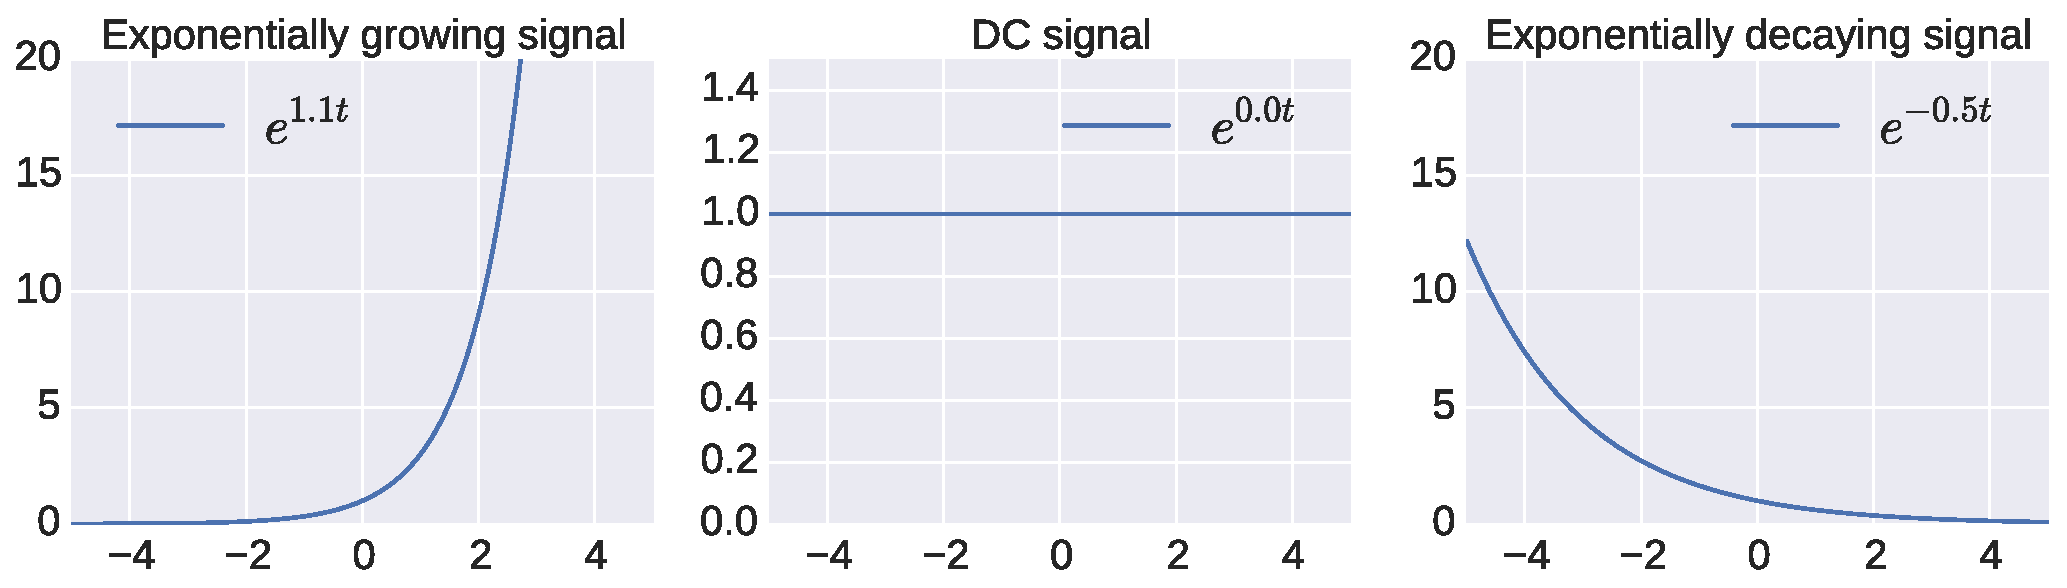
\includegraphics[width=\textwidth]{img/exp.eps}
\end{figure}
\end{frame}

% REAL EXPONENTIALS
\begin{frame}{Real Exponentials}

\textbf{Discrete-time} version
\[ x[n] =  b \left(a\right)^n \]

where, $a, b \in \mathbb{R}$ and $n \in \mathbb{Z}$. $b$ is the amplitude and $a$ is the exponential growth or decay rate.

\begin{figure}
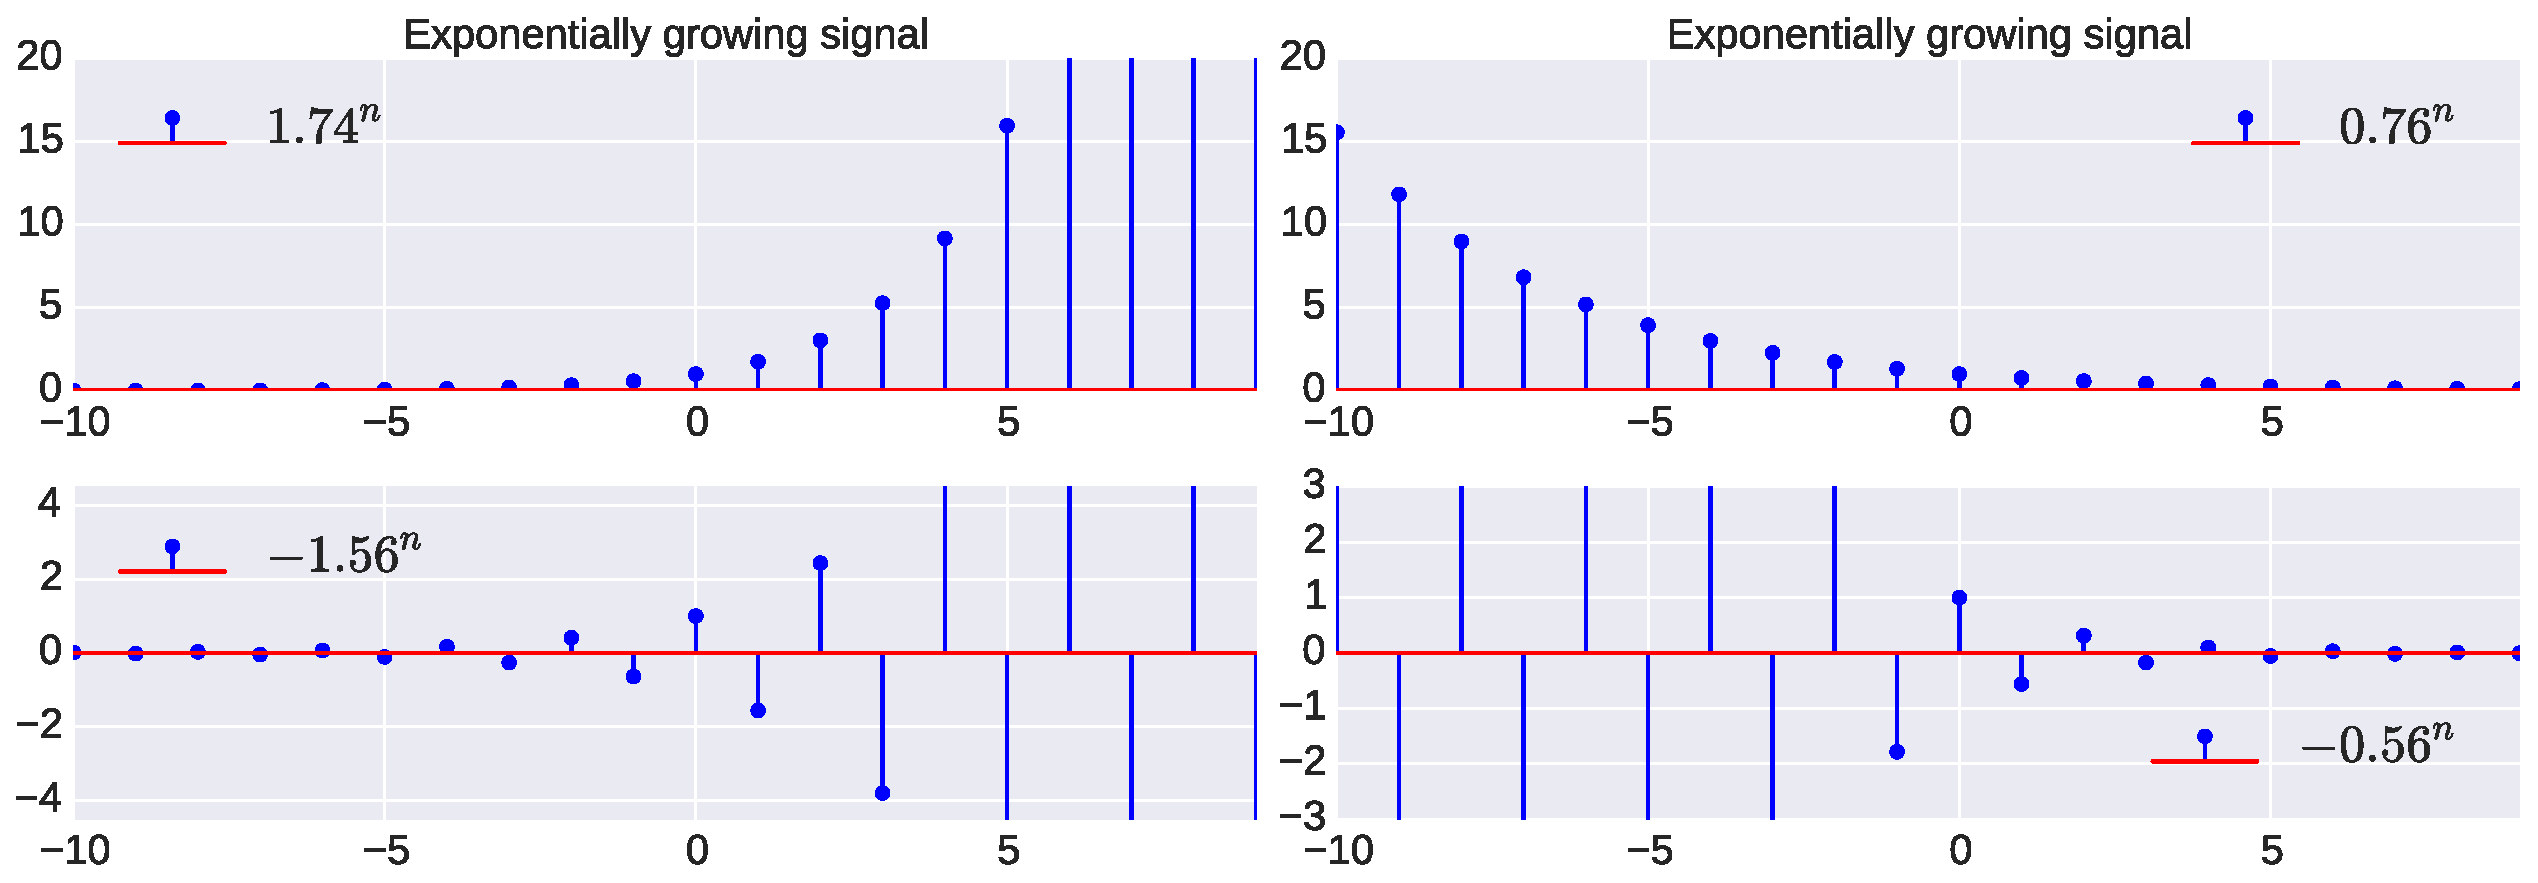
\includegraphics[width=\textwidth]{img/disc_exp.eps}
\end{figure}
\end{frame}

% SINUSOIDAL SIGNALS
\begin{frame}{Sinusoidal signals}
\textbf{Continuous-time} version

\[ x(t) = A \sin \left(\omega t + \phi\right) \]

where, $A$ is the amplitude, $\omega$ is the angular frequency $\left(\mathrm{rad}.\mathrm{sec}^{-1}\right)$, and $\phi$ is the phase angle.

\begin{figure}
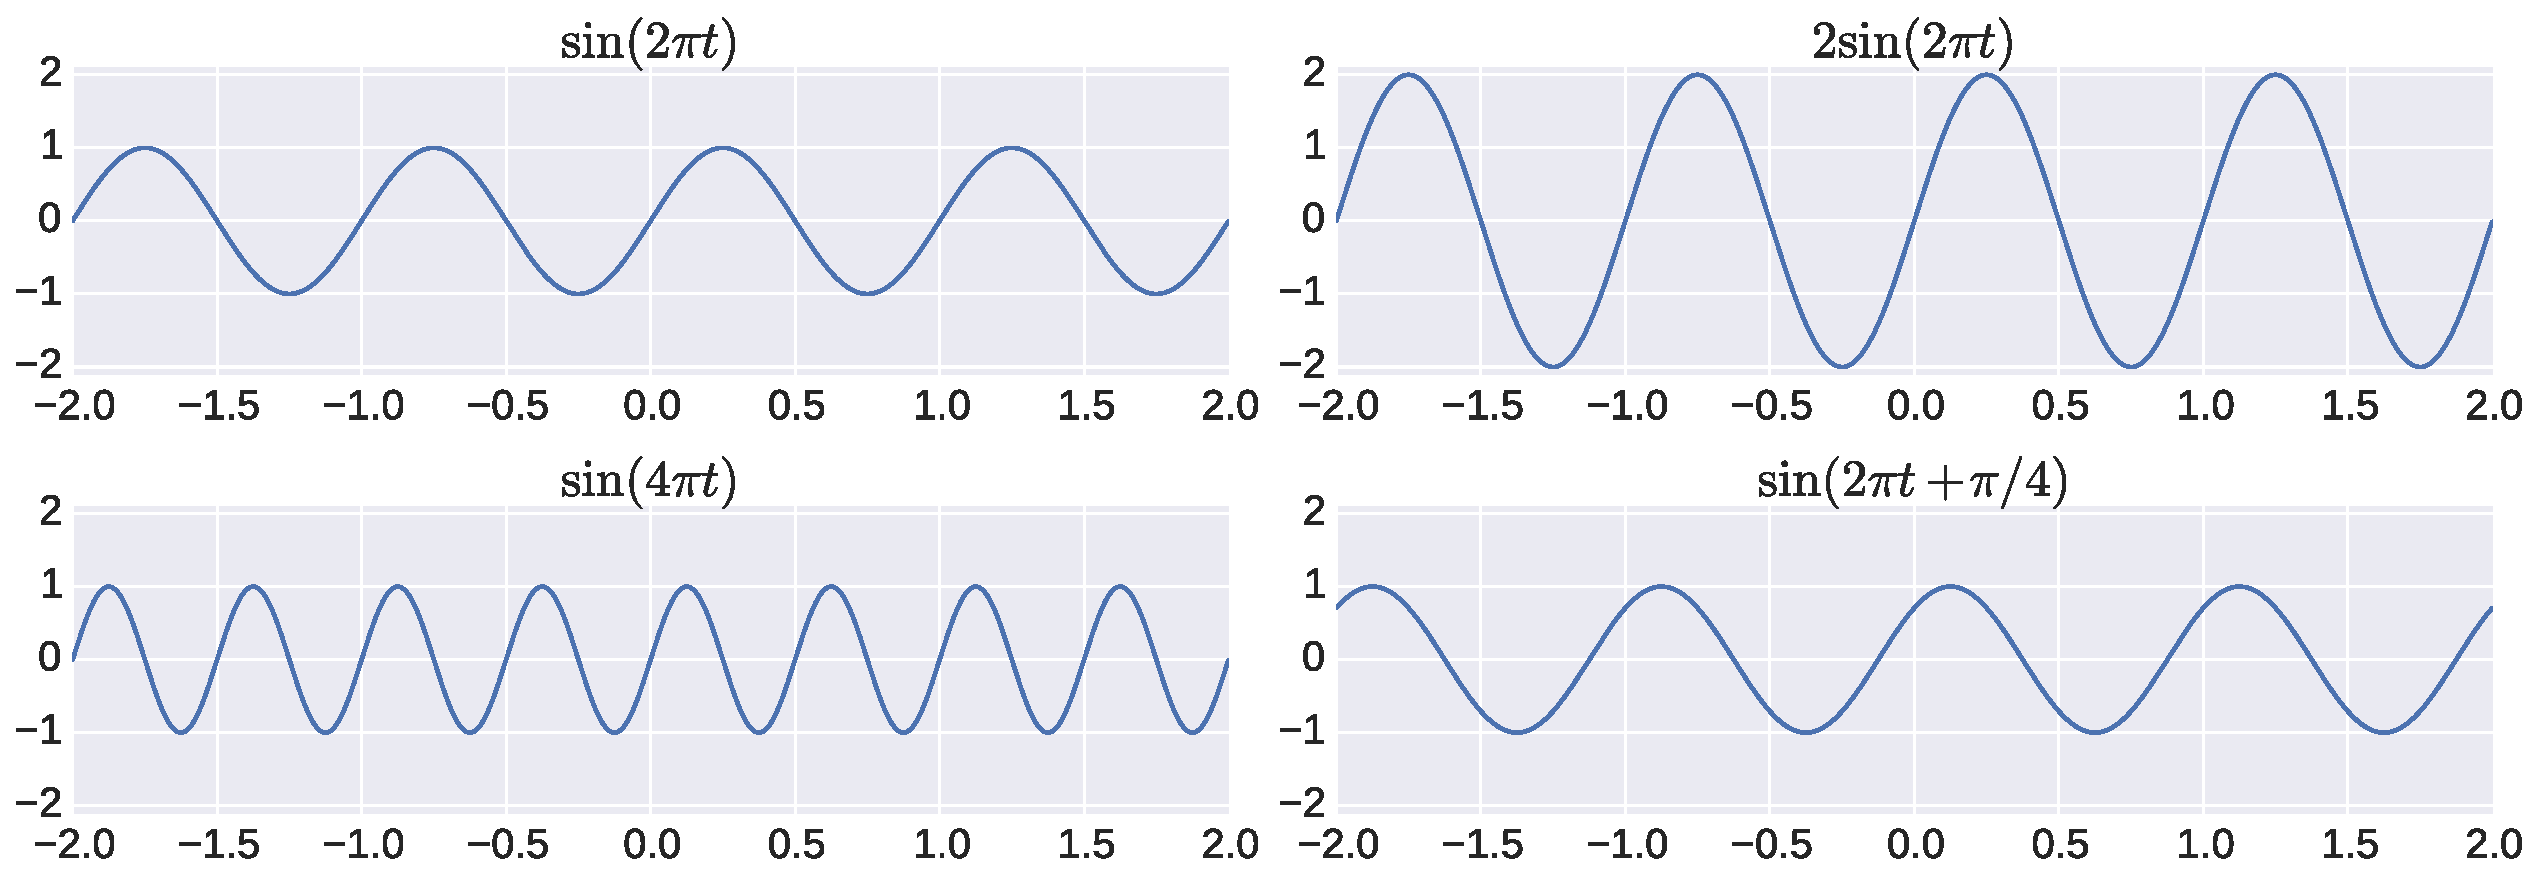
\includegraphics[width=\textwidth]{img/sinu.eps}
\end{figure}

What is the fundamental period of sinusoid?
\end{frame}

% SINUSOIDAL SIGNALS
\begin{frame}{Sinusoidal signals}
\textbf{Discrete-time} version

\[ x[n] = A \sin \left(\Omega n + \phi\right) \]

where, $A$ is the amplitude, $\Omega$ is the digital frequency $\left(\mathrm{rad}.\mathrm{sample}^{-1}\right)$, and $\phi$ is the phase angle.

\begin{figure}
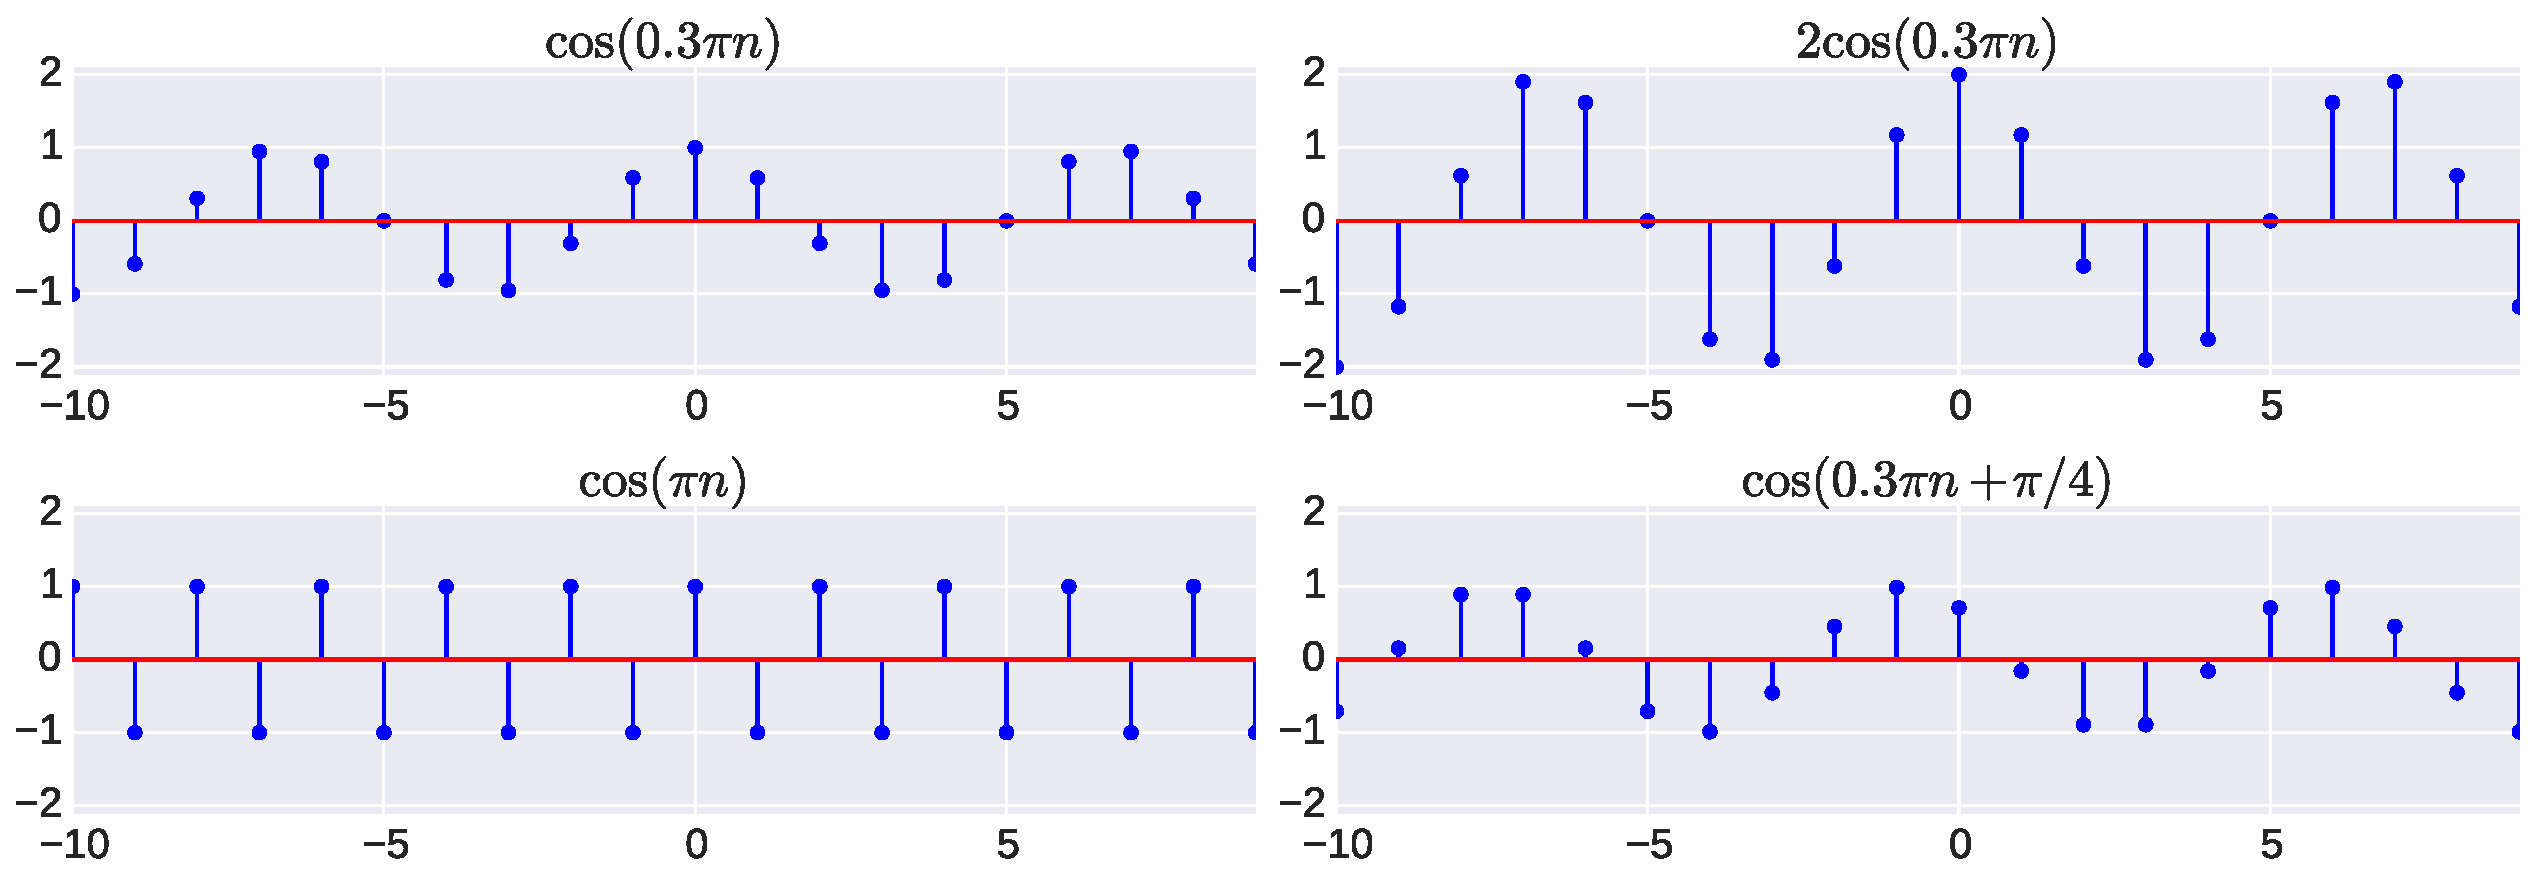
\includegraphics[width=0.8\textwidth]{img/disc_sinu.eps}
\end{figure}

\end{frame}


% SINUSOIDAL SINGALS
\begin{frame}{Sinusoidal signals}\

\textbf{Complex exponential representation of sinusoids}

\[ z = a + jb = \left|z\right|e^{j\theta} = \left|z\right|\cos \theta + j \left|z\right|\sin \theta\]

\begin{figure}
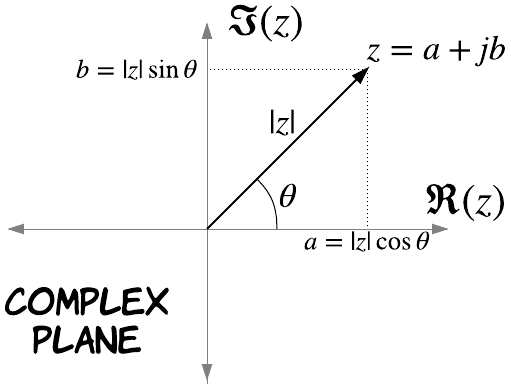
\includegraphics[width=0.5\textwidth]{img/complex_plane.png}
\end{figure}

\[ \cos \theta = \frac{e^{j\theta} + e^{-j\theta}}{2} \,\,\,\,\, \sin \theta = \frac{e^{j\theta} - e^{-j\theta}}{2j}\]

\end{frame}

% EXPONENTIAL SINUSOIDS
\begin{frame}{Exponential sinusoids}
\textbf{Continuous-time} version

Amplitude modulated sinusoids
\[ x(t) = a e^{bt} \sin \left(\omega t + \phi \right), \,\,\,\,\, a, b, \omega, \phi \in \mathbb{R}\]

\begin{figure}
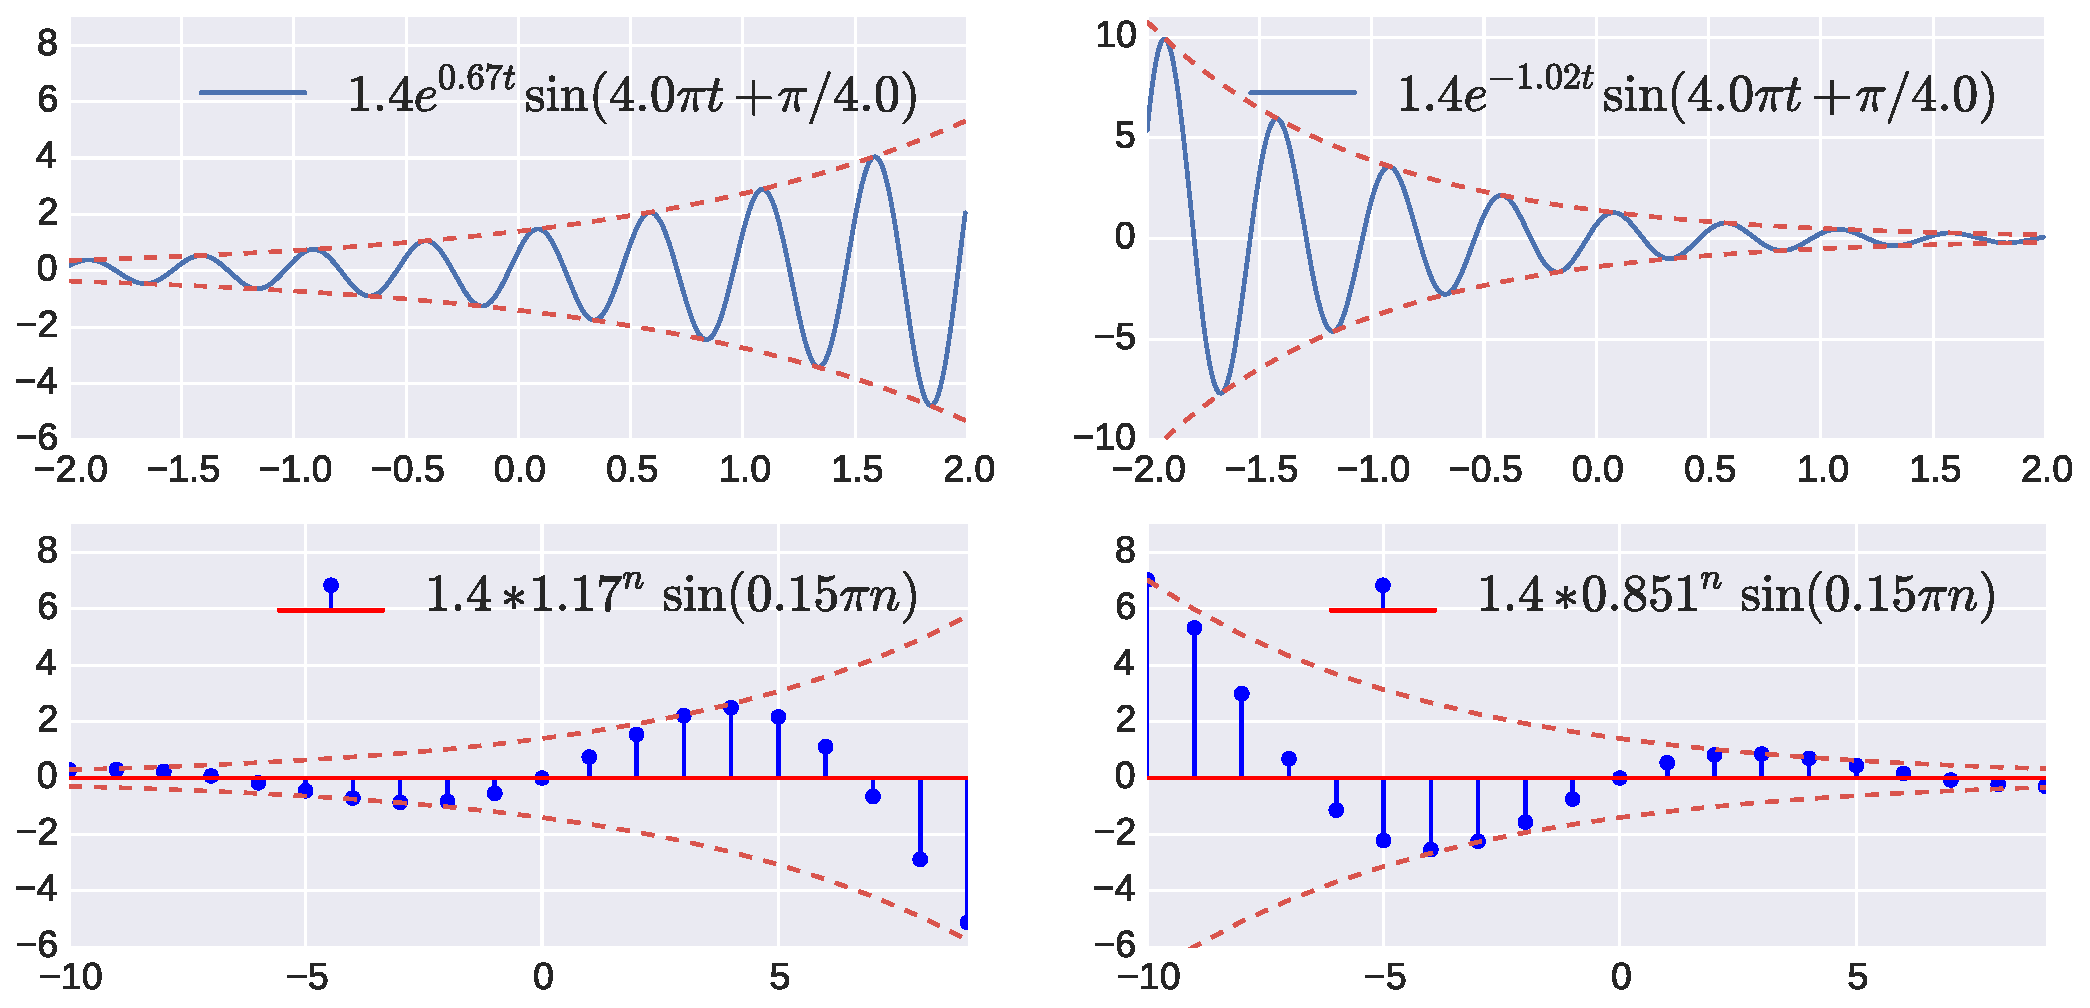
\includegraphics[width=0.8\textwidth]{img/exp_sin.eps}
\end{figure}

\end{frame}

% IMPULSE FUNCTION
\begin{frame}{Impulse function $\delta(t)$, $\delta[n]$}

\textbf{Dirac delta function} $\delta(t)$

\begin{itemize}
\item This is \textbf{\underline{NOT}} a conventional function.
\item It makes sense only when it is used in an integral.
\item It is not characterized by the exact values it takes as a function of the independent variable, but by the following important property.
\[ \int_{a}^{b}\delta (t) = \begin{cases}
1, & 0 \in [a,b] \\
0, & 0 \notin [a, b]
\end{cases} \]
\item It operates like a value selector.
\[ \int_{-\infty}^{\infty}f(t)\delta (t) = f(0), \text{, where $f$ is continuous at } t= 0. \]
\item Impulse function is a very useful theoretical tool for representing: point charges or masses, forces in instantaneous collisions, derivatives of jump discontinuities etc.
\end{itemize}
\end{frame}

% IMPULSE FUNCTION
\begin{frame}{Impulse function $\delta(t)$, $\delta[n]$}
\begin{small}
$\delta(t)$ can be understood through a limiting operation. Let $f_{n}\left(t\right) = \begin{cases}
n, & -\frac{1}{2n} \leq t \leq \frac{1}{2n} \\
0, & \mathrm{Otherwise}
\end{cases}$ and $\int_{-\infty}^{\infty}f_n(t)dt = 1$
\[\int_{-\infty}^{\infty}f_{n}\left(t\right)g\left(t\right)dt = \int_{-\frac{1}{2n}}^{\frac{1}{2n}}ng\left(t\right)dt = g_n = \lim_{n\to\infty}\int_{-\infty}^{\infty}f_{n}\left(t\right)g\left(t\right)dt \]
\[\lim_{n\to\infty}g_{n} = g\left(0\right) = \int_{-\infty}^{\infty}g(t)\delta(t)dt\]
\end{small}
\vspace{-0.5cm}
\begin{figure}
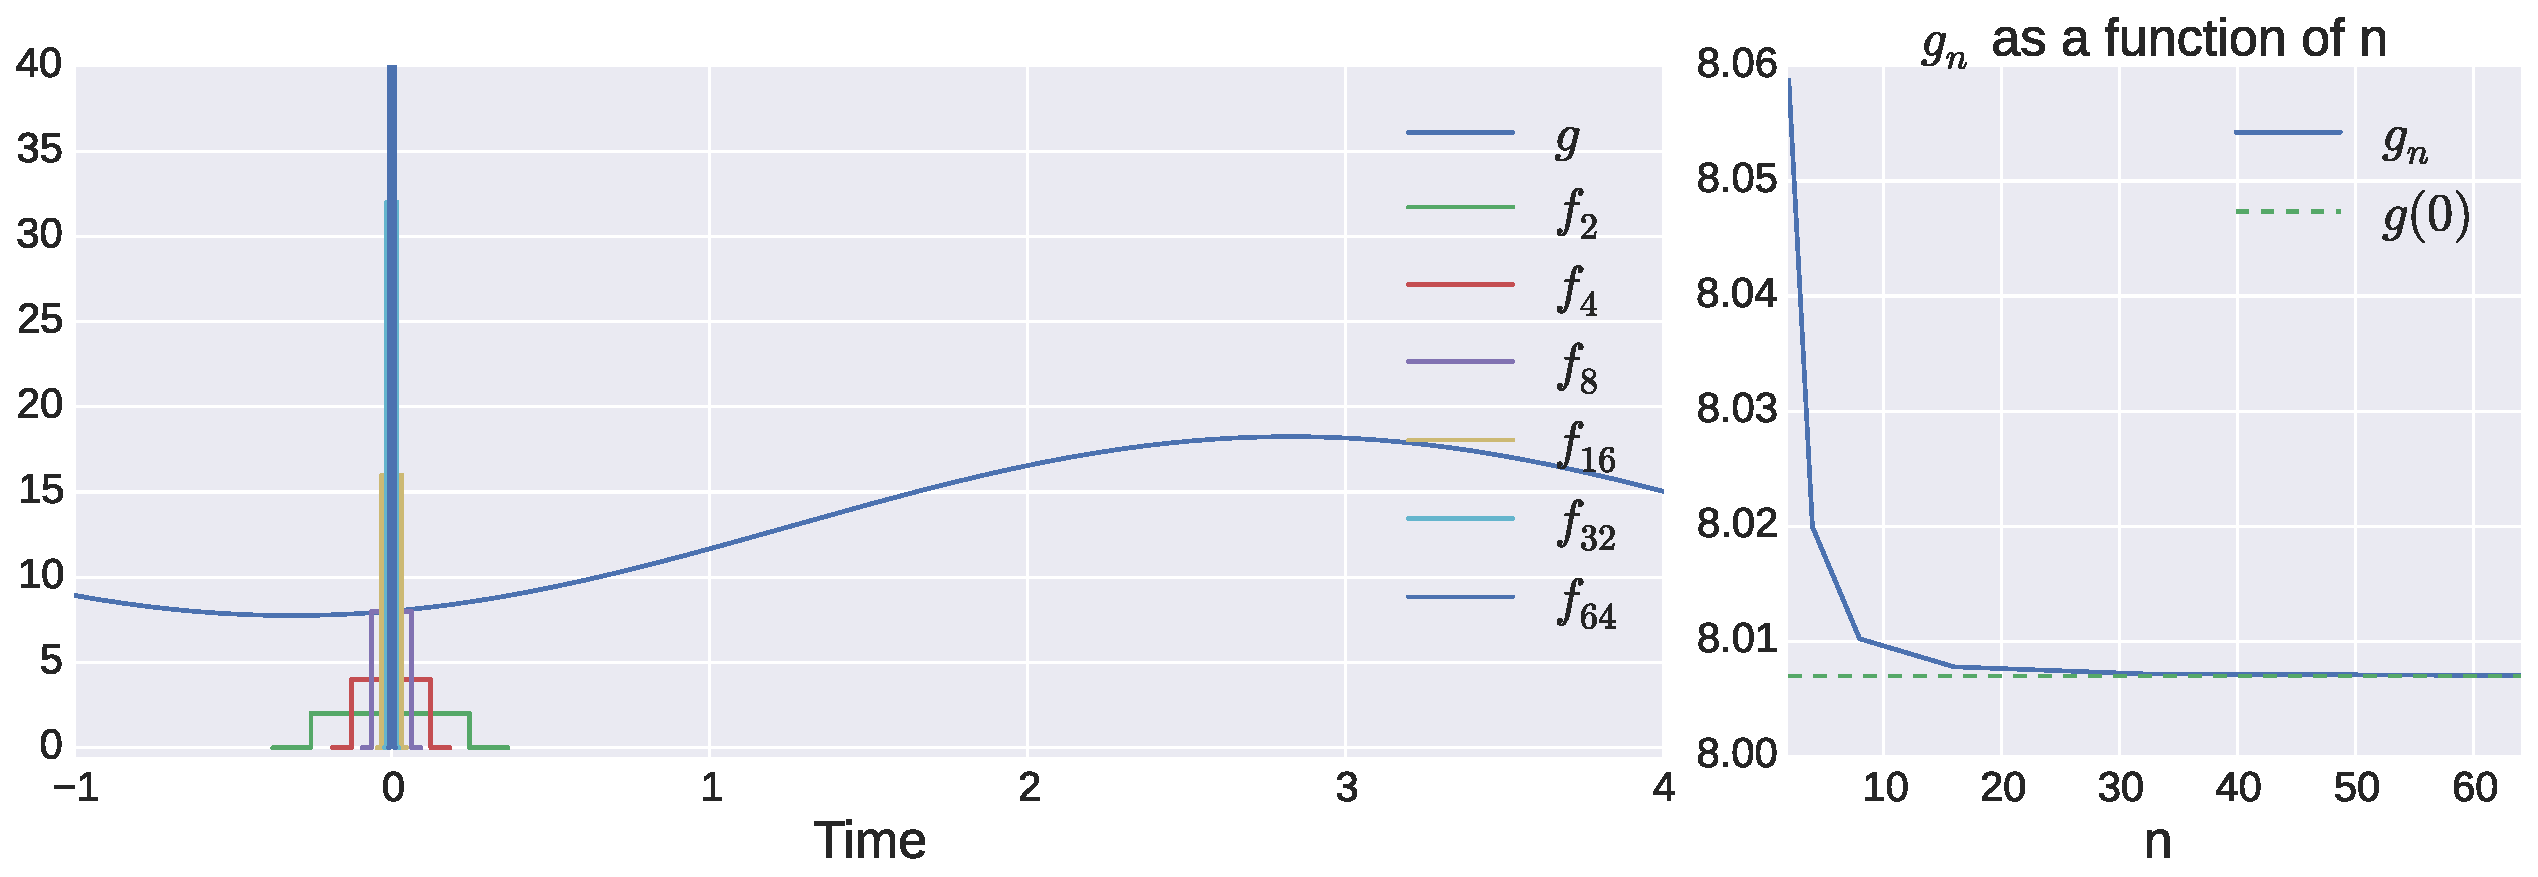
\includegraphics[width=0.8\textwidth]{img/impulse_demo.eps}
\end{figure}
\end{frame}

% IMPULSE FUNCTION
\begin{frame}{Impulse function $\delta(t)$, $\delta[n]$}

\textbf{Kronecker delta function or sequence} $\delta[n]$

\begin{itemize}
\item Very easy to understand unlike the continuous-time version.
\[ \delta[n] = \begin{cases}
1 & n = 0 \\
0 & \mathrm{Otherwise}
\end{cases} \]
\end{itemize}

\begin{figure}
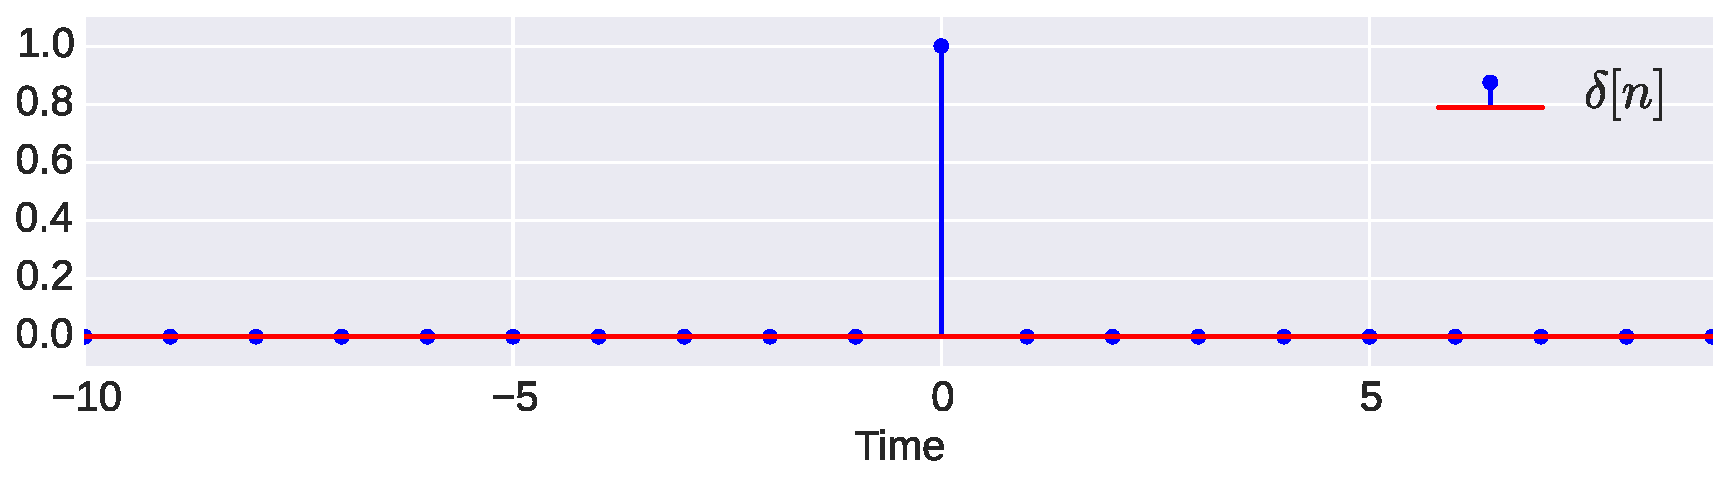
\includegraphics[width=\textwidth]{img/disc_imp.eps}
\end{figure}
\end{frame}

% STEP FUNCTION
\begin{frame}{Step function $1(t), 1[n]$}

Definition of \textbf{continuous-time} unit step function,
\[ 1(t) = \begin{cases}
1 & t > 0\\
\frac{1}{2} & t = 0\\
0 & t < 0
\end{cases}; \,\,\,\,\, 1\lp t\rp = \int_{-\infty}^{t} \delta\lp t\rp dt; \,\,\,\,\,  \frac{d}{dt}1\lp t\rp = \delta\lp t\rp\]
% \[ 1(t) = \int_{-\infty}^{t} \delta(\tau)d\tau \]

\begin{figure}
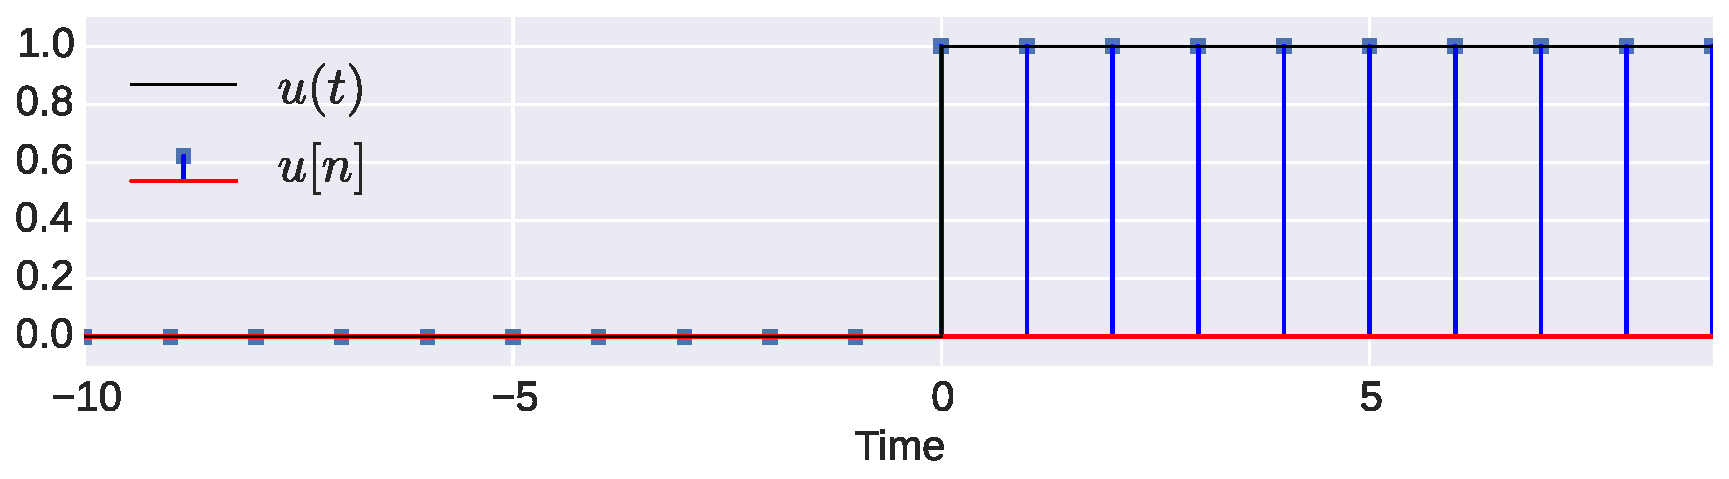
\includegraphics[width=\textwidth]{img/step.eps}
\end{figure}

What is the corresponding definition of the discrete-time unit step function $1[n]$?
\end{frame}


\begin{frame}{Linear System}
\begin{center}
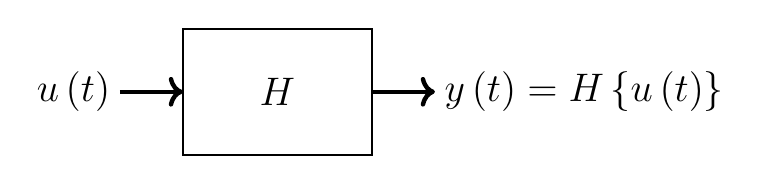
\begin{tikzpicture}[scale=0.8]
    \draw[thick] (0,0) rectangle (3, 2);
    \node at (1.5, 1) {{\Large $H$}};
    \draw[ultra thick, ->] (-1, 1) -- (0, 1);
    \node[left] at (-1, 1) {{\Large $u\lp t\rp$}};
    \draw[ultra thick, ->] (3, 1) -- (4, 1);
    \node[right] at (4, 1) {{\Large $y\lp t\rp = H\lc u\lp t\rp\rc$}};
\end{tikzpicture}
\end{center}
\begin{itemize}
    \item Behavior of dynamic systems can be described mathematically through differential equations (continuous-time systems), or difference equations (discrete-time systems).
    \item A system is \textbf{linear} if, 
    \[ y_1\lp t\rp = H\lc u_1\lp t\rp\rc \text{ and } y_2\lp t\rp = H\lc u_2 \lp t\rp \rc\]
    \[ \implies H\lc a_1x_1\lp t\rp + a_2u_2\lp t\rp \rc = a_1H\lc u_1\lp t\rp\rc + a_2H\lc u_2\lp t\rp \rc = a_1y\lp t\rp + a_2y_2\lp t\rp, \quad a_1, a_2 \in \mathbb{C} \]
\end{itemize}
\end{frame}


\begin{frame}{Time-Invariant System}
\begin{center}
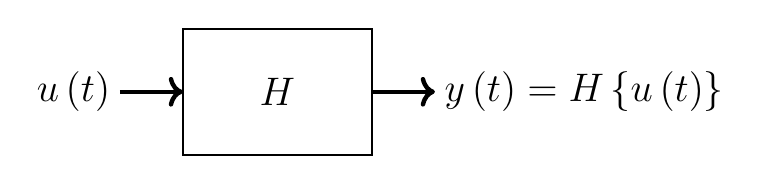
\begin{tikzpicture}[scale=0.8]
    \draw[thick] (0,0) rectangle (3, 2);
    \node at (1.5, 1) {{\Large $H$}};
    \draw[ultra thick, ->] (-1, 1) -- (0, 1);
    \node[left] at (-1, 1) {{\Large $u\lp t\rp$}};
    \draw[ultra thick, ->] (3, 1) -- (4, 1);
    \node[right] at (4, 1) {{\Large $y\lp t\rp = H\lc u\lp t\rp\rc$}};
\end{tikzpicture}
\end{center}
\begin{itemize}
    \item A system is \textbf{time-invariant} if,
    \[ y\lp t\rp = H\lc u\lp t\rp\rc \implies H\lc u \lp t - \tau \rp \rc = y\lp t - \tau \rp \]

    \item Characteristics of the system do not change with time. Time-shifted inputs produce correspondingly time-shifted output.
\end{itemize}
\end{frame}


\begin{frame}{Linear Time-Invariant System}
\begin{center}
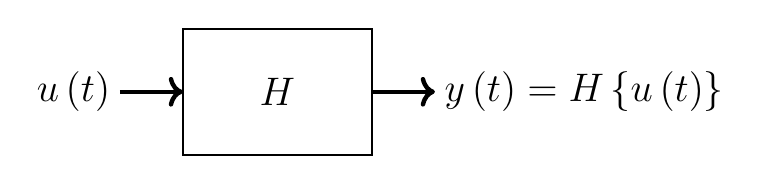
\begin{tikzpicture}[scale=0.8]
    \draw[thick] (0,0) rectangle (3, 2);
    \node at (1.5, 1) {{\Large $H$}};
    \draw[ultra thick, ->] (-1, 1) -- (0, 1);
    \node[left] at (-1, 1) {{\Large $u\lp t\rp$}};
    \draw[ultra thick, ->] (3, 1) -- (4, 1);
    \node[right] at (4, 1) {{\Large $y\lp t\rp = H\lc u\lp t\rp\rc$}};
\end{tikzpicture}
\end{center}
\begin{itemize}
    \item LTI systems: both \textbf{linear} and \textbf{time-invariant}. These are described through constant coefficient linear differential (or difference) equations.

    \item \textbf{Continuous-time}: 
    $$\frac{d^n}{dt^n}y\lp t\rp + a_{1}\frac{d^{n-1}}{dt^{n-1}}y\lp t\rp + \ldots + a_ny\lp t\rp = u\lp t\rp + b_1\frac{d}{dt}u\lp t\rp + \ldots + b_m\frac{d^m}{dt^m}y\lp t\rp $$

    \item \textbf{Discrete-time}:
    $$y\ls k - n\rs + a_1y\ls k - n + 1\rs + \ldots + a_ny\ls k\rs = u\ls k\rs + b_1u\ls k-1\rs + \ldots + b_m u\ls k-m\rs$$
\end{itemize}
\end{frame}


\begin{frame}[t]{Unilateral Laplace Transform}
\begin{itemize}
    \item Unilateral Laplace transform can be used for solving these linear-constatint coefficient differential equations.

    \item Consider a time-domain signal $x\lp t\rp$, such that $x\lp t\rp = 0, \forall t < 0$.    
    \[ \mathcal{L}\lc x\lp t\rp\rc = X\lp s\rp = \int_{0^-}^{\infty} x\lp t\rp e^{-st}dt, \,\,\, s = \sigma + j\omega \]
    where, $X\lp s\rp$ exists only for specific values of $s$, which is called the \textit{region of convergence}.

    \item A time-domain function is converted to a function in the $s$-domain. 

\end{itemize}
\end{frame}


\begin{frame}[t]{Unilateral Laplace Transform}
\begin{itemize}
    \item Unilateral Laplace transform transform $X\lp s\rp$ provides a different way to look at the signal $x\lp t\rp$.

    \item The inverse of a unilateral Laplace transform is often not obtained analytically, but by using a table of Laplace transform pairs $\lp x\lp t\rp, X\lp s\rp\rp$.

\end{itemize}
\vspace{0.5cm}

Evaluate the unilateral Laplace transform of the following:
\begin{enumerate}
    \item $e^{at} \times 1\lp t\rp$
    \item $e^{\lp a + jb\rp t} \times 1\lp t\rp$
    \item $1\lp t\rp$
    \item $\delta \lp t\rp$
    \item $\sin \omega t \times 1\lp t\rp$
\end{enumerate}
\end{frame}

\begin{frame}[t]{Unilateral Laplace Transform}
    
\end{frame}


\begin{frame}[t]{Unilateral Laplace Transform}
    
\end{frame}


\begin{frame}[t]{Unilateral Laplace Transform}
\begin{itemize}
    \item An important property of the unilateral Laplace transform that will be useful in solving differential equations is the Laplace transform on $x'\lp t\rp$,
    \[ \mathcal{L}\lc x'\lp t\rp\rc = sX\lp s\rp - x\lp 0^-\rp \]
    \[ \mathcal{L}\lc x''\lp t\rp\rc = s^2X\lp s\rp - sx\lp 0^-\rp - x'\lp 0^-\rp \]
\end{itemize}
\end{frame}


\begin{frame}[t]{Unilateral Laplace Transform}
Derive and solve the differential equation representing the voltage-current relationship. What is the output for each of the three systems when $v\lp t\rp = v_0 \times 1\lp t\rp$?
\begin{columns}
\begin{column}{0.275\textwidth}
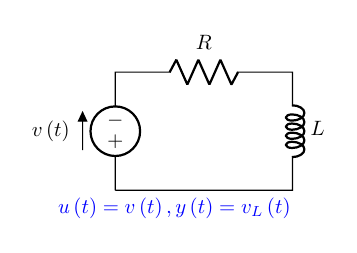
\begin{tikzpicture}[scale=0.75, transform shape]
\path (0,0) coordinate (ref_gnd);
\draw
  (ref_gnd) to[american voltage source= $v\lp t\rp$] ++(0,2)
            to[R=\(R\)] ++(3,0) 
            to[L=\(L\)] ++(0,-2) 
  -- (ref_gnd);
  \node[xshift=1.0cm, below, blue] at (0,0) {$u\lp t\rp = v\lp t\rp, y\lp t\rp = v_L\lp t\rp$};
\end{tikzpicture}
\end{column}
\begin{column}{0.275\textwidth}
\end{column}
\begin{column}{0.275\textwidth}
\end{column}
\end{columns}
\end{frame}


\begin{frame}[t]{Unilateral Laplace Transform}
Derive and solve the differential equation representing the voltage-current relationship. What is the output for each of the three systems when $v\lp t\rp = v_0 \times 1\lp t\rp$?
\begin{columns}
\begin{column}{0.275\textwidth}
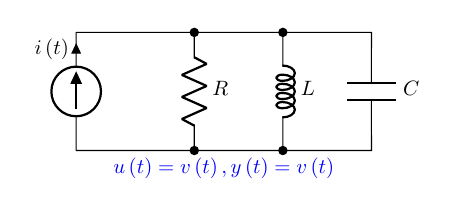
\begin{tikzpicture}[scale=0.75, transform shape]
\path (0,0) coordinate (ref_gnd);
\draw
  (ref_gnd) to[american current source=$i\lp t\rp$] ++(0,2)
            -- ++(2,0)   to[R=\(R\)] ++(0,-2) -- (ref_gnd) 
  ++(2,2)   -- ++(1.5,0) to[L=\(L\)] ++(0,-2) -- ++(-1.5,0)
  ++(1.5,2) -- ++(1.5,0) to[C=\(C\)] ++(0,-2) -- ++(-1.5,0);
\fill[color=black] (ref_gnd)++(2,0)   circle[radius=0.08];
\fill[color=black] (ref_gnd)++(3.5,0) circle[radius=0.08];
\fill[color=black] (ref_gnd)++(2,2)   circle[radius=0.08];
\fill[color=black] (ref_gnd)++(3.5,2) circle[radius=0.08];
\node[xshift=2.5cm, below, blue] at (0,0) {$u\lp t\rp = v\lp t\rp, y\lp t\rp = v\lp t\rp$};
\end{tikzpicture}
\end{column}
\begin{column}{0.275\textwidth}
\end{column}
\begin{column}{0.275\textwidth}
\end{column}
\end{columns}
\end{frame}


\begin{frame}{Impulse Response}
\begin{itemize}
    \item In case we do not know the exact composition of the system, and only have access to the input and output ports, i.e. we can manipulate the input and observe (measure) the output. How can we characterize the system in this case?
    \vspace{0.2cm}
    \begin{center}
    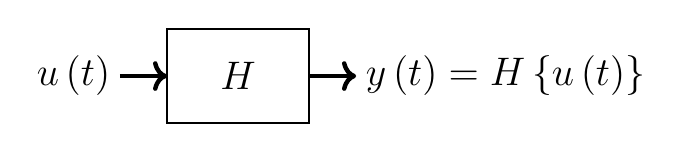
\begin{tikzpicture}[scale=0.6]
        \draw[thick] (0,0) rectangle (3, 2);
        \node at (1.5, 1) {{\Large $H$}};
        \draw[ultra thick, ->] (-1, 1) -- (0, 1);
        \node[left] at (-1, 1) {{\Large $u\lp t\rp$}};
        \draw[ultra thick, ->] (3, 1) -- (4, 1);
        \node[right] at (4, 1) {{\Large $y\lp t\rp = H\lc u\lp t\rp\rc$}};
    \end{tikzpicture}
    \end{center}
    \vspace{0.2cm}

    \item When the system $H$ is (or approximately) LTI, there is a nice way to characterize the system.

    \item If we know the system output $\lc w_i\lp t\rp\rc_{i=1}^n$ for a set of signals, $\lc v_i\lp t\rp\rc_{i=1}^n$, then system output for an arbitrary input $u\lp t\rp = \sum_{i=1}^n a_i v_i\lp t - \tau_i\rp$ is,
    \[ y\lp t\rp = H\lc u\lp t\rp\rc = H\lc \sum_{i=1}^n a_i v_i\lp t - \tau_i\rp\rc = \sum_{i=1}^n a_i w_i\lp t - \tau_i\rp \]
\end{itemize}
\end{frame}


\begin{frame}{Impulse Response}
\begin{center}
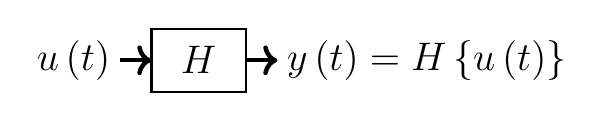
\begin{tikzpicture}[scale=0.4]
    \draw[thick] (0,0) rectangle (3, 2);
    \node at (1.5, 1) {{\Large $H$}};
    \draw[ultra thick, ->] (-1, 1) -- (0, 1);
    \node[left] at (-1, 1) {{\Large $u\lp t\rp$}};
    \draw[ultra thick, ->] (3, 1) -- (4, 1);
    \node[right] at (4, 1) {{\Large $y\lp t\rp = H\lc u\lp t\rp\rc$}};
\end{tikzpicture}
\end{center}

\begin{itemize}    
    \item Ideally, $V = \lc v_i\lp t\rp \rc_{i=1}^n$ is chosen to allows us to represents a wide range of signals using $V$.
    
    \item The are two popular choices: \textbf{(a)} $\delta\lp t \rp$; and \textbf{(b)} $e^{st}$.

    \item A signal $u\lp t\rp$ can be represented in the following form,

    \[ u\lp t\rp = \int_{-\infty}^{\infty} u\lp \tau \rp \delta\lp \tau - t\rp d\tau \]
    
    The representation arises as the limit of a sequence of functions are are approximated by rectangular pulse,
    \[ u\lp t \rp = \lim_{\Delta \to 0} \sum_{n=-\infty}^{\infty} u\lp t_n \rp \lp \frac{1\lp t - t_n\rp - 1\lp t - t_{n+1}\rp}{\Delta}\rp \Delta; \,\,\, n\Delta \leq t < \lp n+1\rp\Delta  \]   
\end{itemize}
\end{frame}


\begin{frame}{Impulse Response}
\begin{center}
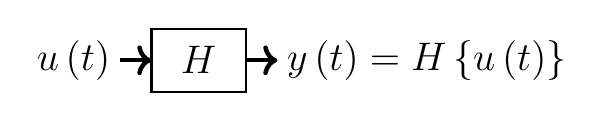
\begin{tikzpicture}[scale=0.4]
    \draw[thick] (0,0) rectangle (3, 2);
    \node at (1.5, 1) {{\Large $H$}};
    \draw[ultra thick, ->] (-1, 1) -- (0, 1);
    \node[left] at (-1, 1) {{\Large $u\lp t\rp$}};
    \draw[ultra thick, ->] (3, 1) -- (4, 1);
    \node[right] at (4, 1) {{\Large $y\lp t\rp = H\lc u\lp t\rp\rc$}};
\end{tikzpicture}
\end{center}
\begin{itemize} 
    \item The output of the system to $u\lp t\rp$ is given by,
    \[ y\lp t\rp = H\lc \int_{-\infty}^{\infty} u\lp \tau \rp \delta\lp \tau - t\rp d\tau \rc = \int_{-\infty}^{\infty} u\lp \tau \rp H\lc \delta\lp \tau - t\rp  \rc d\tau \]
    \[ y\lp t\rp = \int_{-\infty}^{\infty} u\lp \tau \rp h\lp \tau - t\rp d\tau = u\lp t\rp * h\lp t\rp = h\lp t\rp * u\lp t\rp \]
    \[ h\lp t\rp = H\lc \delta\lp t\rp \rc \]
\end{itemize}
\end{frame}


\begin{frame}[t]{Impulse Response}
\begin{itemize}
    \item $h\lp t\rp$ is the \textit{impulse response} of the LTI system $H$. \textbf{Note:} The system must be at rest when the impulse is applied at the input, i.e. the output must be zero $y(t) = 0, \forall t < 0$
    \item The output of $H$ to an input $u\lp t\rp$ is obtained through the \textit{convolution} between $u\lp t\rp$ and $h\lp t\rp$.
\end{itemize}
\end{frame}


% IMPULSE RESPONSE AND SYSTEM PROPERTIES
\begin{frame}{Convolution Integral}
\begin{figure}
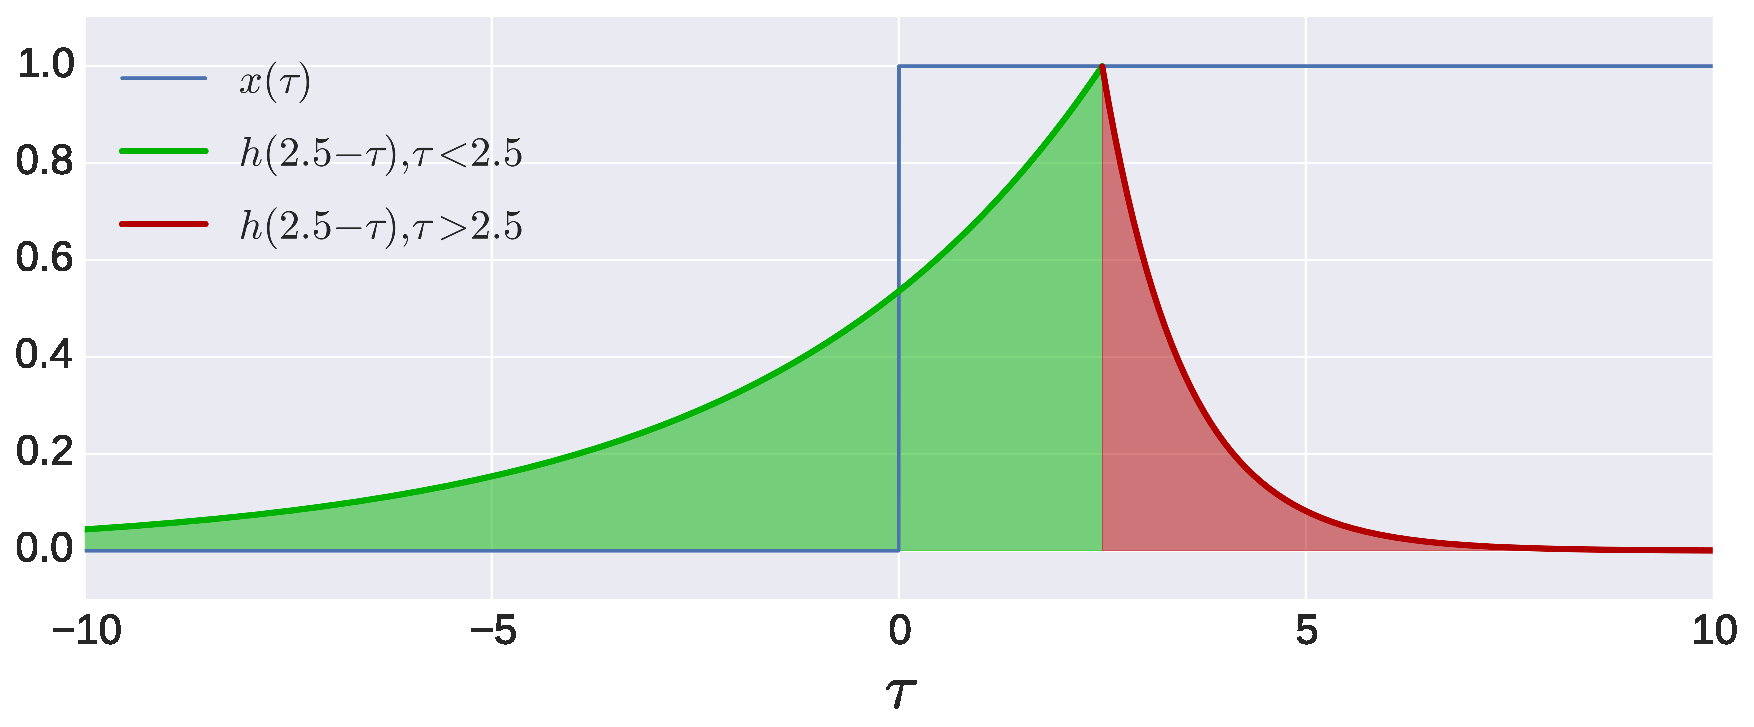
\includegraphics[width=0.7\textwidth]{img/imp_resp_mech.eps}
\end{figure}
\begin{small}
$h(t) = \begin{cases}
e^{t} & t < 0 \\
e^{-0.25t} & t \geq 0 \\
\end{cases}$ and $x(t) = 1(t)$. $h\lp t\rp$ acts as a weighting function. It evlauates the present output by weighting the present, past and future input values.

\[ \begin{cases}
h(t), \forall t < 0 & \text{Weightage for the future} \\
h(0) & \text{Weightage for the present} \\
h(t), \forall t > 0 & \text{Weightage for the past} \\
\end{cases}
\]
\end{small}
\end{frame}


\begin{frame}{Convolution Integral}
What is the output $y\lp t\rp$ of a system $H$ with the following impulse response $h\lp t\rp$ and input $u\lp t\rp$?
\vspace{0.3cm}
\begin{columns}
\begin{column}{0.45\textwidth}
\textbf{1. }$h\lp t\rp = e^{-at}1\lp t\rp$
\begin{itemize}
    \item $u\lp t\rp = 1\lp t\rp$
    \item $u\lp t\rp = \delta\lp t - 1\rp + 0.5 \delta\lp t - 5\rp$
\end{itemize}
\vspace{0.3cm}
\textbf{2. }$h\lp t\rp = 1\lp t\rp - 1\lp t - 1\rp$
\begin{itemize}
    \item $u\lp t\rp = e^{-t}1\lp t\rp$
    \item $u\lp t\rp = 1\lp t - 2\rp + 1\lp t - 5\rp$
\end{itemize}
\end{column}

\begin{column}{0.5\textwidth}
% \vspace{0.3cm}
\textbf{3. }$h\lp t\rp = e^{-at}1\lp t\rp + e^{bt}1\lp -t\rp$
\begin{itemize}
    \item $u\lp t\rp = 1\lp t\rp$
    \item $u\lp t\rp = \delta\lp t - T_2\rp + \delta\lp t - T_3\rp$
\end{itemize}
\vspace{0.3cm}
\textbf{4. }$h\lp t\rp = 1\lp t\rp$
\begin{itemize}
    \item $u\lp t\rp = 1\lp t\rp$
    \item $u\lp t\rp = e^{-at}1\lp t\rp$
\end{itemize}
\end{column}
\end{columns}
\end{frame}

\begin{frame}[t]
\end{frame}


\begin{frame}{Transfer function}
\begin{itemize}    
    \item \textbf{Output of a LTI system to $e^{st}$}:
    \[ y\lp t\rp = h\lp t\rp * e^{st} = \int_{-\infty}^{\infty} h\lp \tau \rp e^{s\lp t - \tau\rp}  d\tau = \lp \int_{-\infty}^{\infty} h\lp \tau \rp e^{-s\tau}  d\tau \rp e^{st} \]
    \[ y\lp t\rp = H\lp s\rp e^{st} \implies H\lp s\rp = \frac{\text{Response to } e^{st}}{e^{st}}\] 

    \item $e^{st}$ are the \textit{eigenfunctions} of LTI systems, and their corresponding \textit{eigenvalue} is $H\lp s\rp$. For these functions, convolution $h\lp t\rp * e^{st}$ is simplified to multiplication $H\lp s\rp \times e^{st}$.

    \item $H\lp s\rp$ is called the transfer function of the LTI system. This is the \textit{bilateral} Laplace transform of the impulse response $h\lp t\rp$. This becomes the unilateral Laplace transform when $h\lp t\rp = 0, \forall t < 0$.
\end{itemize}
\end{frame}


\begin{frame}{Transfer function}
\begin{itemize}    
    \item In general, the Laplace transform of a general linear constant coefficient different equation with zero initial conditions would be of the following form.
    \[ s^nY\lp s\rp + a_1s^{n-1}Y\lp s\rp + \ldots + a_nY\lp s\rp = U\lp s\rp + b_1sU\lp s\rp + \ldots + b_ms^mU\lp s\rp \]
    \[ \frac{Y\lp s\rp}{U\lp s\rp} = \frac{b_ms^m + b_{m-1}s^{m-1} + \ldots + b_{1}s + 1}{s^n + a_1s^{n-1} + \ldots + a_{n-1}s + a_n}  = \frac{B\lp s\rp}{A\lp s\rp} = H\lp s\rp\]

    \[ H(s) = b_m\frac{\left(s - z_1\right)\left(s - z_2\right)\cdots\left(s - z_m\right)}{\left(s - p_1\right)\left(s - p_2\right)\cdots\left(s - p_n\right)} \]

    \item The roots of $B\lp s\rp$ and $A\lp s\rp$ are the \textit{zeros} and \textit{poles} of the system. 

    \item Poles of the system determine the stability of the system, in the BIBO sense -- Bounded Input, Bounded Output.

    \item $H$ is stable in BIBO sense, if
    \[ \lv u\lp t\rp \rv < M_u < \infty \implies \lv y\lp t\rp\rv = H\lc u\lp t\rp\rc < M_y < \infty \]
\end{itemize}
\end{frame}


\begin{frame}[t]{Transfer function}
Derive the transfer function and impulse response for the following systems.
\begin{columns}
\begin{column}{0.275\textwidth}
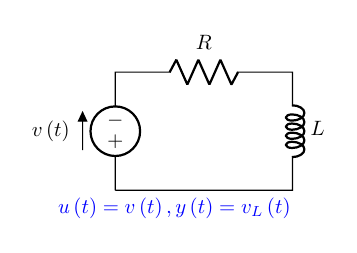
\begin{tikzpicture}[scale=0.75, transform shape]
\path (0,0) coordinate (ref_gnd);
\draw
  (ref_gnd) to[american voltage source= $v\lp t\rp$] ++(0,2)
            to[R=\(R\)] ++(3,0) 
            to[L=\(L\)] ++(0,-2) 
  -- (ref_gnd);
  \node[xshift=1.0cm, below, blue] at (0,0) {$u\lp t\rp = v\lp t\rp, y\lp t\rp = v_L\lp t\rp$};
\end{tikzpicture}
\end{column}

\begin{column}{0.275\textwidth}
\end{column}

\begin{column}{0.45\textwidth}
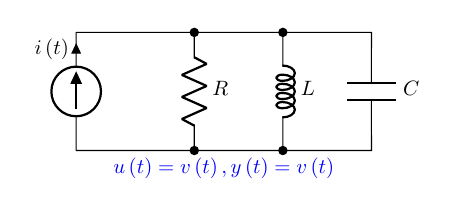
\begin{tikzpicture}[scale=0.75, transform shape]
\path (0,0) coordinate (ref_gnd);
\draw
  (ref_gnd) to[american current source=$i\lp t\rp$] ++(0,2)
            -- ++(2,0)   to[R=\(R\)] ++(0,-2) -- (ref_gnd) 
  ++(2,2)   -- ++(1.5,0) to[L=\(L\)] ++(0,-2) -- ++(-1.5,0)
  ++(1.5,2) -- ++(1.5,0) to[C=\(C\)] ++(0,-2) -- ++(-1.5,0);
\fill[color=black] (ref_gnd)++(2,0)   circle[radius=0.08];
\fill[color=black] (ref_gnd)++(3.5,0) circle[radius=0.08];
\fill[color=black] (ref_gnd)++(2,2)   circle[radius=0.08];
\fill[color=black] (ref_gnd)++(3.5,2) circle[radius=0.08];
\node[xshift=2.5cm, below, blue] at (0,0) {$u\lp t\rp = v\lp t\rp, y\lp t\rp = v\lp t\rp$};
\end{tikzpicture}
\end{column}
\end{columns}
\end{frame}


\begin{frame}[t]{z transform}
\begin{itemize}    
    \item The discrete-time equivalent of the Laplace transform is the $z$- transform. The unilateral z-transform is defined as,
    \[ X\lp z\rp = \mathcal{Z}\lc x\ls k\rs\rc = \sum_{k=0}^{\infty} x\ls k\rs z^{-k} \]
    $X\lp z\rp$ exists only for specific set of vaues of $z$, which is called the \textit{region of convergence}.

    \vspace{0.5cm}
    Evaluate the unilateral z transform of the following: (i) $a^k \times 1\ls k\rs$; (ii) $\cos \Omega k \times 1\ls k\rs$; (iii) $1\ls k\rs$; (iv) $\delta \ls k\rs$
\end{itemize}
\end{frame}


\begin{frame}[t]{z transform}
\begin{itemize}
    \item Unilateral z-transform can be used for solving linear constant coefficient difference equations.
    \item If $x\ls k\rs \xleftrightarrow{\mathcal{Z}} X\lp z\rp$, then
    \[ \mathcal{Z}\lc x\ls k - 1\rs\rc = zX\lp z\rp + x\ls -1\rs \]
\end{itemize}
\end{frame}


\begin{frame}{Impulse Response}
\begin{center}
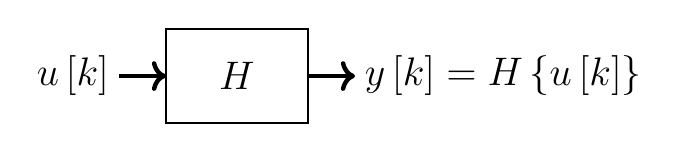
\begin{tikzpicture}[scale=0.6]
    \draw[thick] (0,0) rectangle (3, 2);
    \node at (1.5, 1) {{\Large $H$}};
    \draw[ultra thick, ->] (-1, 1) -- (0, 1);
    \node[left] at (-1, 1) {{\Large $u\ls k\rs$}};
    \draw[ultra thick, ->] (3, 1) -- (4, 1);
    \node[right] at (4, 1) {{\Large $y\ls k\rs = H\lc u\ls k\rs\rc$}};
\end{tikzpicture}
\end{center}

\begin{itemize}
    \item Any discrete-time signal can be represented as a linear combination of time-shifted impulse sequences,
    \[ x\ls k\rs = \sum_{l=-\infty}^{\infty} x\ls l\rs \delta \ls k - l\rs \]

    \item The output of the system $H$ to any input sequence is given by,
    \[ y\ls k\rs = H\lc u\ls k\rs\rc = \sum_{l=-\infty}^{\infty} x\ls l\rs H\lc \delta \ls k - l\rs\rc = \sum_{l=-\infty}^{\infty} x\ls l\rs h\ls k - l\rs \]
    \[ y\ls k\rs = x\ls k\rs * h\ls k \rs \]
    This is the \textit{convolution sum}, and $h\ls k\rs$ is the \textit{impulse response} of the system $H$.
\end{itemize}
\end{frame}

\begin{frame}[t]{Convolution Sum}
What is the output $y\ls k\rs$ of a system $H$ with the following impulse response $h\ls k\rs$ and input $u\ls k\rs$?
\vspace{0.3cm}
\begin{columns}
\begin{column}{0.45\textwidth}
\textbf{1. }$h\ls k\rs = a^k1\ls k\rs$
\begin{itemize}
    \item $u\ls k\rs = 1\ls k\rs$
    \item $u\ls k\rs = \delta\ls k - 1\rs + 0.5 \delta\ls k - 5\rs$
\end{itemize}
\vspace{0.3cm}
\textbf{2. }$h\ls k\rs = 1\ls k\rs - 1\ls k - 5\rs$
\begin{itemize}
    \item $u\ls k\rs = a^{k}1\ls k\rs$
    \item $u\ls k\rs = 1\ls k - 2\rs + 1\ls k - 8\rs$
\end{itemize}

\end{column}

\begin{column}{0.5\textwidth}
% \vspace{0.3cm}
\textbf{3. }$h\ls k\rs = a^k1\ls k\rs + b^k1\ls k\rs$
\begin{itemize}
    \item $u\ls k\rs = 1\ls k\rs$
    \item $u\ls k\rs = \delta\ls k - N_1\rs + \delta\ls k - N_2\rs$
\end{itemize}

\vspace{0.3cm}
\textbf{4. }$h\ls k\rs = 1\ls k\rs$
\begin{itemize}
    \item $u\lss k\rs = 1\ls k\rs$
    \item $u\ls k\rs = a^{k}1\ls k\rs$
\end{itemize}
\end{column}
\end{columns}
\end{frame}


\begin{frame}{Transfer function}
\begin{center}
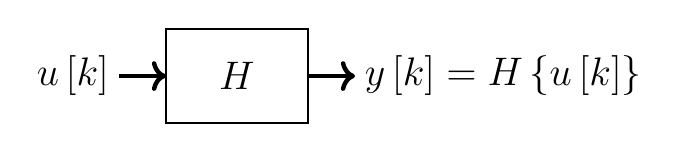
\begin{tikzpicture}[scale=0.6]
    \draw[thick] (0,0) rectangle (3, 2);
    \node at (1.5, 1) {{\Large $H$}};
    \draw[ultra thick, ->] (-1, 1) -- (0, 1);
    \node[left] at (-1, 1) {{\Large $u\ls k\rs$}};
    \draw[ultra thick, ->] (3, 1) -- (4, 1);
    \node[right] at (4, 1) {{\Large $y\ls k\rs = H\lc u\ls k\rs\rc$}};
\end{tikzpicture}
\end{center}

\begin{itemize}
    \item \textbf{Output of a LTI system to $z^k$}: 
    \[ y\ls k\rs = h\ls k\rs * z^k = \sum_{l=-\infty}^{\infty} h\ls l\rs z^{\lp k - l\rp} = \lp \sum_{l=-\infty}^{\infty} h\ls l\rs z^{-l} \rp z^k = H\lp z\rp z^k\]

    \item $H\lp z\rp$ is the transfer function of the system $H$, which is the z-transform of the impulse response $h\ls k\rs$.

    \item $z^k$ is the \textit{eigenfunction} of a discrete-time LTI system, and $H\lp z\rp$ is the corresponding \textit{eigenvalue}.
\end{itemize}
\end{frame}


\begin{frame}{Transfer function}
\begin{itemize}    
    \item In general, z-transform of a general linear constant coefficient difference equation with zero initial conditions would be of the following form.
    \[ z^{-n}Y\lp z\rp + a_1z^{-\lp n -1\rp}Y\lp z\rp + \ldots + a_nY\lp z\rp = U\lp z\rp + z^{-1}b_1U\lp z\rp + \ldots + b_mz^{-m}U\lp z\rp \]
    \[ \frac{Y\lp z\rp}{U\lp z\rp} = \frac{b_mz^{-m} + b_{m-1}z^{-\lp m-1\rp} + \ldots + b_{1}z^{-1} + 1}{z^{-n} + a_1z^{-\lp n-1\rp} + \ldots + a_{n-1}z^{-1} + a_n}  = \frac{B\lp z\rp}{A\lp z\rp} = H\lp z\rp\]

    \[ H(s) = b_mz^{\lp n - m\rp}\frac{\lp z - \hat{z}_1\rp\lp z - \hat{z}_2\rp\cdots\lp z - \hat{z}_m\rp}{\lp z - p_1\rp\lp z - p_2\rp\cdots\lp z - p_n\rp} \]

    \item Poles of the system determine the stability of the system, in the BIBO sense -- Bounded Input, Bounded Output.

    \item $H$ is stable in BIBO sense, if
    \[ \lv u\ls k\rs \rv < M_u < \infty \implies \lv y\ls k\rs\rv = H\lc u\ls k\rs\rc < M_y < \infty \]
\end{itemize}
\end{frame}


\begin{frame}[t]{Transfer function}
Derive the transfer function and impulse response for the following systems.
\begin{itemize}
    \item $y\ls k\rs + 0.5y\ls k - 1\rs = u\ls k\rs$
    \item $y\ls k\rs + y\ls k - 1\rs + 0.5y\ls k - 2\rs = u\ls k\rs$
    \item $y\ls k\rs + 0.5y\ls k - 2\rs = u\ls k - 2\rs$
    \item $y\ls k\rs + 0.5y\ls k - 2\rs = 2u\ls k\rs + u\ls k - 2\rs$
\end{itemize}
\end{frame}


\end{document}